% JuliaCon proceedings template
\documentclass{juliacon}
\setcounter{page}{1}

\begin{document}

% **************GENERATED FILE, DO NOT EDIT**************

\title{UnROOT.jl - Data I/O for High-Energy Physics in Julia}

\author[1]{Jerry Ling}
\author[2]{Tamás Gál}
\affil[1]{Harvard University}
\affil[2]{Erlangen Centre for Astroparticle Physics}

\keywords{Julia, HEP, JuliaHEP, JuliaCon, RNTuple, ROOT, ROOT File}

\hypersetup{
pdftitle = {UnROOT.jl - Data I/O for High-Energy Physics in Julia},
pdfsubject = {JuliaCon 2022 Proceedings},
pdfauthor = {Jerry Ling, Tamás Gál},
pdfkeywords = {Julia, HEP, JuliaHEP, JuliaCon, RNTuple, ROOT, ROOT File},
}



\maketitle

\begin{abstract}
    \verb|RNTuple| is the upcoming primary data storage solution at the Large Hadron Collider (LHC)
    experiments and other high-energy physics (HEP) experiments going forward. Aside from many
    technical upgrades from the \verb|TTree| object, \verb|RNTuple| also is the first time
    \verb|.root| file committed to specification.\cite{rntuple_2023}

    In this paper we present the latest
    development in \verb|UnROOT.jl| that enables both the reading and writing of complex
    table-like data structures in Julia with \verb|RNTuple|. At the moment this is the most complete
    3rd party libraries that can read and write \verb|RNTuple| data outside of \verb|C++ ROOT|.

\end{abstract}

\section{Introduction}
Before \verb|RNTuple|, \verb|UnROOT.jl| has been focues on read-only workload when it comes to
\verb|.root| files.\cite{unroot_2022} This has yielded real-world and sometimes large-scale
application of Julia in physics data analysis in the field of HEP. However, the lack of writing
capability has stopped experiments and individual users from integration Julia workflow into
existing data pipelines or replace legacy components that are increasingly difficult to maintain.

With the introduction of \verb|RNTuple|, Julia can now be used in scopes larger than end-user
analysis. In the context of the larger JuliaHEP movement, as outlined in our community white paper
\cite{juliahep_whitepaper}, this is a significant milestone in the foundational data I/O dimension
of the ecosystem.

\subsection{History}
ROOT is a data analysis framework developed by CERN and is widely used in the HEP community. Among
many things, it also defines a file format, the \verb|.root| file, which is used to store data in
the order of exabytes as of writing. The \verb|TTree| object inside the \verb|.root| file has been
the primary storage format for the last two decades.

When \verb|UnROOT.jl| was first introduced, it was a read-only library that can read \verb|.root|
and we focused on performance, thread-safety and ease of use, since we recognized the technical
merit and potential of Julia programming language as a great fit for the various needs of the HEP
community. This has proven fruitful, the performance of \verb|UnROOT.jl| has been competitive even
when compared to the \verb|C++ ROOT| library and scales well with memory-shared parallelism which is
natively supported by Julia.
\cite{chep_2023}.

\section{RNTuple in UnROOT.jl}
While there exists unique challenges in reading and writing, it is useful to briefly introduce
RNTuple's approach generally before going into the details of the implementation in
\verb|UnROOT.jl|. 

The most important difference between \verb|TTree| and \verb|RNTuple| is the schema.

In
\verb|TTree|, the schema is directly mapped to the physical storage, which means that the
user-facing columns (known as \verb|TBranch|) are 1-to-1 with the physical storage. This is
illustrated in Figure \ref{fig:ttree_schema}. This designed had a number of problems, one of which
is if a column is very complex, the implementation has to invent ad-hoc ways to squeeze the data
into the storage unit, which hurts performance and makes the file format 
implementation-specific.


\begin{figure}[h]
\centerline{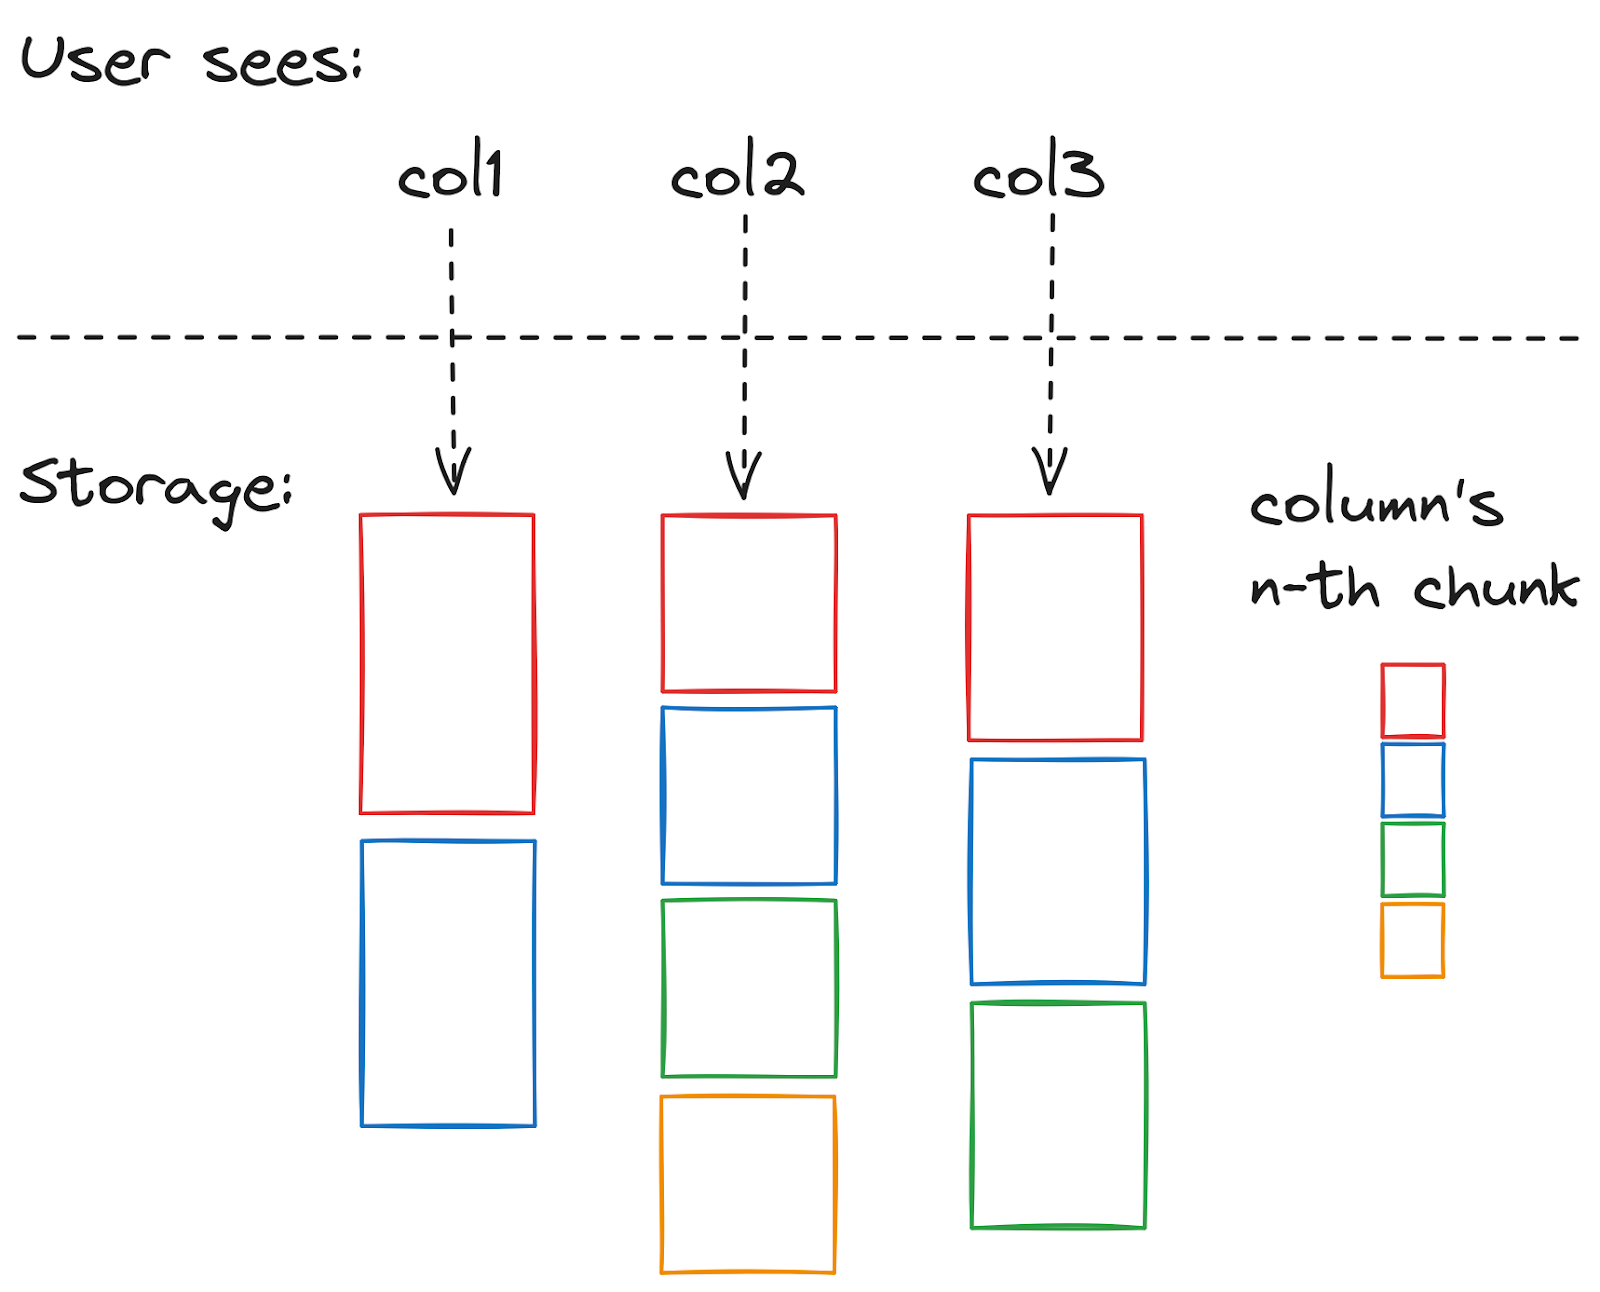
\includegraphics[width=6cm]{ttree_schema.png}}
\caption{Schematics of the schema (or there lack of) in TTree, the user-faceing branches are 1-to-1
with the physical storage.}
	\label{fig:ttree_schema}
\end{figure}

By contrast, in \verb|RNTuple|, the user-facing types are decoupled from the physical storage,
mediated by a schema system composed of \verb|field|s and
\verb|column|s.\footnote{\url{https://root.cern/doc/master/md_tree_2ntuple_2v7_2doc_2BinaryFormatSpecification.html}}
This allows better compression efficiency and uniform schema composition rule, and is crucial to the
universal composability of the file format. This is illustrated in Figure \ref{fig:rntuple_schema}.



\begin{figure}[h]
\centerline{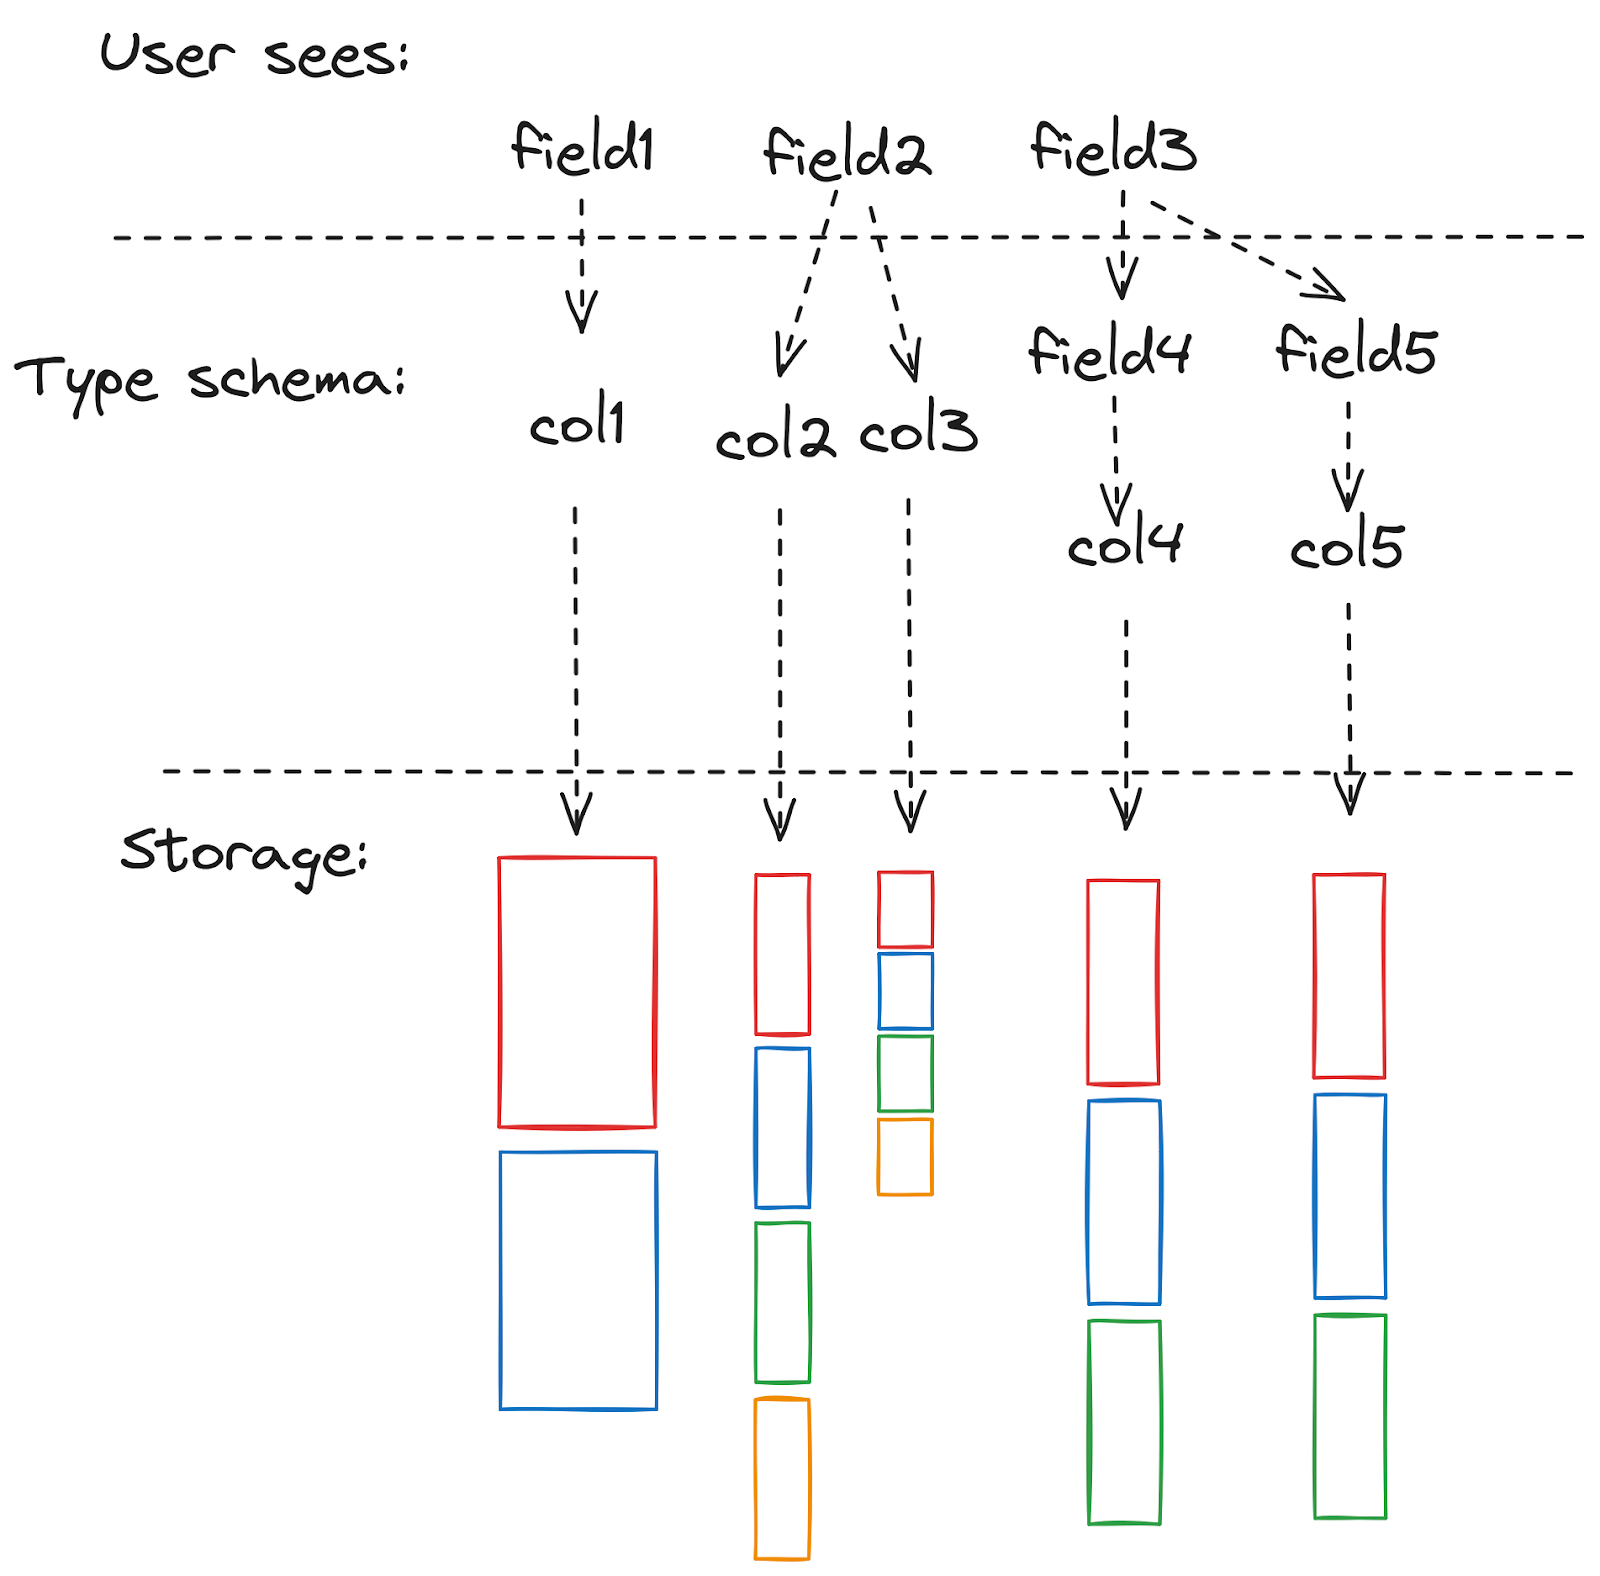
\includegraphics[width=6cm]{rntuple_schema.png}}
\caption{Schematics of the schema in RNTuple, notice how the user-facing fields are no longer 1-to-1
with the physical storage.}
	\label{fig:rntuple_schema}
\end{figure}

We would like to highlight two key aspects of our implementation, first is the assembling (for
reading) and decomposing (for writing) of the schema using Julia's type system, and second is the
flexible \verb|Table.jl|-compatible interface provided by \verb|UnROOT.jl| which enables user to
analize the physics data using the larger Julia data science ecosystem.

\subsection{Type-space manipulation with Julia type system}
The basic strategy for reading and writing is the following:
\begin{enumerate}
    \item Define base case implementations for the basic types, such as all the primitive types,
        the vector types, the struct types, and the union types.
    \item For more complex types, recursively build or decompose the types via Juila's dispatch
        system.
\end{enumerate}

For example, the following is the definition of some of the field types in \verb|UnROOT.jl|:
\begin{lstlisting}[
    language = Julia, 
    numbers=left, 
    label={lst:unroot_schema}, 
    caption={Definition of some RNTuple field types in UnROOT.jl for reading}
]
struct VectorField{O, T}
    offset_col::O
    content_col::T
end
struct StructField{N, T}
    content_cols::T
end
struct UnionField{S,T}
    switch_col::S
    content_cols::T
end
\end{lstlisting}

These basic types can then compose into arbitrary complex types, such as the following:
\begin{lstlisting}[
    language = Julia, 
    numbers=left, 
    label={lst:unroot_example}, 
    caption={Example of a single user-facing field seen in ATLAS PHYSLITE format}
]
AntiKt4TruthDressedWZJetsAux: => Struct
  |- :m => Vector
  |       |- :offset => Leaf{Index64}(col=132)
  |       |- :content => Leaf{Float32}(col=133)
  |- :pt => Vector
  |        |- :offset => Leaf{Index64}(col=126)
  |        |- :content => Leaf{Float32}(col=127)
  |- :eta => Vector
  |         |- :offset => Leaf{Index64}(col=128)
  |         |- :content => Leaf{Float32}(col=129)
\end{lstlisting}

\subsection{Table.jl interface for downstream users}

As is the tradition of many Julia packages, \verb|UnROOT.jl| strives to be as composable as
possible, this means two things:
\begin{enumerate}
    \item Read: shouldn’t force special data structure onto users

    \item Write: shouldn’t require users to prepare their input into a narrow set of types

\end{enumerate}

For reading, we provide \verb|Table.jl| compatible interface, which means that in additional the
very performant for-loop style, user can also conduct physics analysis using columnar style via
\verb|DataFrame| and \verb|Query.jl| for example:

\begin{lstlisting}[
    language = Julia, 
    numbers=left, 
    label={lst:unroot_table}, 
    caption={Example of processing RNTuple using DataFrames.jl and Query.jl}
]
@from evt in rntuple begin
    @where length(evt.Jet_pt) > 6
    @let njets=length(evt.Jet_pt)
    @let njets40=sum(evt.Jet_pt.>40)
    @select {njets=njets, njets40, evt.MET_pt}
    @collect DataFrame
end
\end{lstlisting}

For writing, we again accept anything that \verb|istable()| according to the \verb|Table.jl|. In
addition, we also dispatch on types such as \verb|AbstractVector| for each column, which means that
we don't require user to prepare their input into a pre-defined, \verb|UnROOT.jl|-specific container:
\begin{lstlisting}[
    language = Julia, 
    numbers=left, 
    label={lst:unroot_write}, 
    caption={Example of different user types that will result in the same normalized type after
    writing to RNTuple}
]
using ArraysOfArrays: VectorOfVectors
x = [[1,2], [2,3,4]]
x = [1:2, 2:4]
x = VectorOfVectors([1:2, 2:4])
\end{lstlisting}

\section{Conclusion}
In a major update to the \verb|UnROOT.jl| package, we have added the capability to read and write
RNTuple, which is a first among non-official libraries and a significant milestone to achieve the
larger goals of JuliaHEP in enabling physicists to express and solve problems more effectively.

% **************GENERATED FILE, DO NOT EDIT**************

\bibliographystyle{juliacon}
\bibliography{ref.bib}


\end{document}

% Inspired by the International Journal of Computer Applications template
